\documentclass[10pt]{article}

\addtolength{\oddsidemargin}{-.875in}
\addtolength{\evensidemargin}{-.875in}
\addtolength{\textwidth}{1.75in}

\addtolength{\topmargin}{-.875in}
\addtolength{\textheight}{1.75in}

\openup 1em

%macro for commenting
\usepackage{color}
\newcommand{\leo}[1]{{\color{blue}{\it leo: #1}}}

% \newcommand{\Xbeta}{ X_i \theta}
\newcommand{\xbeta}{ x_i \beta}
\newcommand{\xtheta}{ x_i \theta}
% \newcommand{\xbetaij}{ x_{ij}^T \theta}
\newcommand{\sgamma}{s_{ij}^T\gamma_i}

\usepackage[round]{natbib}

\usepackage{rotating}
\usepackage{graphicx}
\usepackage{subcaption}

\usepackage{float}
\usepackage{bbm}

\usepackage{amsthm,amsmath} 
\usepackage{amssymb}
\usepackage{subcaption}
\usepackage{nicefrac}

\newtheorem{theorem}{Theorem}
\newtheorem{lemma}{Lemma}
\newtheorem{corollary}{Corollary}
\newtheorem{remark}{Remark}


\usepackage{algorithm}
\usepackage{algpseudocode}

%\usepackage{mhequ}
\newcommand{\be}{\begin{equation}\begin{aligned}}
\newcommand{\ee}{\end{aligned}\end{equation}}
\newcommand{\bb}[1]{\mathbb{#1}}
\newcommand{\mc}[1]{\mathcal{#1}}
\DeclareMathOperator{\Binom}{Binomial}
\DeclareMathOperator{\No}{No}
\DeclareMathOperator{\PG}{PG}
\DeclareMathOperator{\IG}{Inverse-Gamma}
\DeclareMathOperator{\Ga}{Gamma}
\DeclareMathOperator{\Bern}{Bernoulli}
\DeclareMathOperator{\U}{Uniform}
\DeclareMathOperator{\Poi}{Poisson}
\DeclareMathOperator{\NB}{NB}
\DeclareMathOperator{\cov}{cov}
\DeclareMathOperator{\var}{var}
\DeclareMathOperator{\diag}{diag}
\DeclareMathOperator{\Diag}{Diag}
\newcommand{\KL}[2]{\textnormal{KL}\left(#1 \parallel #2\right)}

\DeclareMathOperator{\bigO}{\mc O}



\thispagestyle{empty}
\baselineskip=28pt

\title{\textbf{Extrinsic Prior for Simple and Efficient\\ Bayesian Modeling with Parameter Constraints}}
%\author{Leo Duan, David Dunson}
\date{}
\begin{document}

\maketitle


{\bf Abstract:} Parameter constraints are very common in statistical models. Examples include linear inequality, parameter ordering, monotonicity, orthogonality, etc. Bayesian approach is quite useful for probabilistic modeling and uncerntainty quantification in the constrained space. Although specific solutions have been made for different constraints, it is challenging to incorporate them in advanced applications, such as modeling with non-parametric assumption or high-dimensional data. In this paper, we propose a simple and general solution by first replacing constraints with strongly informative prior. Through this {\it extrinsic} prior, the parameters are relaxed to a less restrictive space, where conventional tools such as Hamiltonian Monte Carlo are utilized to obtain approximate posterior. Then these posteriors can be easily projected back to the constrained space for exact solution. This approach is very efficient and applicable to a wide range of problems with equality and inequality constraints. The generality allows more families of prior to be chosen for the constrained parameters, and simplifies the adoption of multiple constraints for desired property such as identifiability. Theory is developed and novel statistical applications under constraints are illustrated.
\vskip 12pt

%\baselineskip=12pt
%\par\vfill\noindent
{\noindent  KEY WORDS:  Constraint violation; Space embedding; Monotone Dirichlet; Orthogonal Gaussian processes; Posterior mixing; Projected Markov chain}
%\par\medskip\noindent
%\clearpage\pagebreak\newpage
\pagenumbering{arabic}

\section{Introduction}

Constraints are very common in statistical modeling. In applied domain, modeling assumptions often require some constraint. For example, in functional data analysis related to degenerative disease, it is common to assume the curve need to satisfy certain shape constraint such as monotonicty \citep{lin2014monogp}. In stastical optimization, constraints such as orthonormality are also routinely used to ensure identifiability of the model \citep{uschmajew2010well}. In manifold modeling, a large class of manifolds can be viewed as sub-manifolds of a more conventional space (e.g. Euchlean space), embedded via different constraints.

These constraints can cause substantial modeling difficulty. When constraints are applied on the data, they could generate an intractable integral with the parameter in the likelihood, leading to a ``doubly intractable'' problem. Several successful solutions have been proposed to address this issue \citep{murray2012mcmc,rao2016data}.
On the other hand, there is a clear lack of general and simple solution, when the constraints are applied on the parameters. In frequentist optimization literature, the use of Lagrange and Karush-Kuhn-Tucker multipliers provides a means to obtain point estimate under the equality and inequality constraints \citep{boyd2004convex}. But due to the space constraint, the standard asympotic approximation for variance estimation usually do not hold. Therefore, a Bayesian approach would be more approriate to quantify the uncertainty. Ideally, one would assign prior on a constraint support, then utilize standard toolbox such as Markov chain Monte carlo (MCMC) to obtain posterior sample on this space. However, this turns out to be very challenging.

To assign prior on the constraint space, the available families of distribution are often quite limited. For example, for othornormal matrices on the Stiefel manifold, the matrix von Mises-Fisher distribution \citep{khatri1977mises} is one of the only few choices. For regression under linear inequality constraints, only until recently a tractable prior is proposed for the polyhedral region set by the inequailities \citep{danaher2012minkowski}. Alternatively, \cite{gelfand1992bayesian} proposed a truncation strategy by first considering common unrestricted distribution, then assigning zero support outside the constraint region. Accordingly, the posterior estimation proceeds in first generating unrestricted proposals using Gibbs sampling, then only accepting those inside the constraint space. Although this approach allows using a more general class of prior distribution, the drawback is that the unrestricted proposal can have significant mass outside the constraint region, resulting in a high rejection rate.

To meet the constraints, efficient computation is elusive and often demands substantial efforts to develop. And often it can be disrupted by slight complication such as hierarchical structure or additional constraint. For example, stick-breaking parameterization is commonly used in probability simplex modeling, in order to circumvent the constraint of vertices summing to $1$. However, its computational efficency can be broken by additional structure constraint, such as the ordering of the simplex, which is useful in reducing the label switching problem in mixture modeling \citep{diebolt1994estimation}. As another example, in multiway tensor factorization, orthonormality is useful to induce good posterior mixing in estimating factor matrices. This largely relies on the sampler of Bingham-von Mises-Fisher distribution \citep{hoff2016equivariant}. However, when there is symmetry in the slices of tensor (commonly in population of undirected networks), at least two factors would be the same. This disrupts the closed form of the posterior, demanding new rejection sampling algorithm to be developed. The Bayesian manifold modeling also faces the same quadmire. Hamiltonian Monte Carlo accomodating the geometric structure of the manifold have been developed \citep{girolami2011riemann,byrne2013geodesic}, but the computation is intensive and mixing is suboptimal. These challenges prohibit a good utilization of constraints in statistics.

We propose to solve this problem by viewing the constrigent constraints as a limiting case of a strongly informative prior, referred as extrisic prior. We then relax the effective support of the prior to the neighbor of the constraint space, allowing approximate posterior to be collected efficiently via Hamiltonian Monte Carlo directly in Euchledean space. The imperfection of approximation can be corrected by an efficient reconstruction of an exact Markov chain after projection. The proposed approach is simple to implement and can be automatically carried out via software such as STAN. Theoretic studies are conducted and substantial improvement is shown in simulations and data application.




\section{Method}

We consider a parameter $\theta$ in a constrained space $\mc D$. The space $\mc D$ can be high- or infinite-dimensional. The common Bayesian approach assigns a prior for $\theta$ in $\mc D$, denoted by $\pi_{0,\mc D}(\theta)$. Typically, priors are chosen for computational conveniences so that the posterior can be easily sampled, strictly from $\mc D$. We refer these strategies as intrinsic approaches. Clearly, the choices of priors and constraints one can impose are very limited. Instead, we consider extrinsic approaches, where one sample random variables in the larger space $\mc R$ where $\mc D\in \mc R$, then use them as approximate or proposal in rejection sampling. We first provide an probabilistic justification for extrinsic approaches.


Assuming $\pi_{0,\mc D}(\theta)$ is proper $\int_{\mc D} \pi_{0,\mc D}(\theta) <\infty$, then this prior can be viewed as a conditional density, based on another density $\pi_{0,\mc R}(\theta)$ associated with $\mc R$:

\begin{equation}
\begin{aligned}
\pi_{0,\mc D}(\theta)= \pi_{0,\mc R}(\theta \mid \theta \in \mc D) = \frac{ \pi_{0,\mc R}(\theta) \mathbbm{1}_{\theta\in \mc D} }{ \int_{\mc D}  \pi_{0,\mc R}(\theta) d\theta}.
\end{aligned}
\end{equation}
where $\mathbbm{1}_{\theta \in \mc D}=1$ when $\theta \in \mc D$, $0$ otherwise. Note $\pi_{0,\mc R}(\theta)$ can be improper, as along as $\pi_{0,\mc R}(\theta) \mathbbm{1}_{\theta\in \mc D}$ is proper. Then the posterior can be obtained via:

\begin{equation}
\begin{aligned}
\label{exact_posterior}
\pi(\theta \mid y, \theta \in \mc D) = \frac{ L(\theta;y)\pi_{0,\mc D}(\theta)}{\int_{\mc D} L(\theta;y)\pi_{0,\mc D}(\theta) d\theta } = \frac{ L(\theta;y)\pi_{0,\mc R}(\theta) \mathbbm{1}_{\theta\in \mc D} }{\int_{\mc D} L(\theta;y)\pi_{0,\mc R}(\theta) d\theta },
\end{aligned}
\end{equation}
where the last equality holds because $\int_{\mc D}  \pi_{0,\mc R}(\theta) d\theta$ is a finite constant. Utilizing this form, \cite{gelfand1992bayesian} suggested generating proposal in $\mc R$ based on $L(\theta;y)\pi_{0,\mc R}(\theta)$, then accepting it when it falls in $\mc D$. When the probability $\Pr(\theta\in \mc D \mid y) / \Pr(\theta\in \mc R \setminus D \mid y) \approx 0$, this leads to significant amount of rejections.

%Throughout this section, we use one example to illustrate the embedding and the method. Consider an {\it ordered} $(d-1)$-simplex. The parameter is a $d$-dimensional probability vector $\theta=\{p_1,\ldots,p_d\}$ with $p_1\ge p_2 \ge \ldots \ge p_d$. Its space $\mc D$ is embedded in $[0,1]^d$ via $d-1$ inequality constraints $p_{i+1}-p_i \le 0$ for $i=1,\ldots, d-1$ and one equality constraint $\sum_{i=1}^{d} p_i-1 = 0$. Alternatively, one can view the space $\mc D$ as embedded in a broader space $\mathbb R^d$, via additional $d$ identity inequalities $p_i \ge 0$ for $i=1,\ldots,d$; however this is not necessary since in general, constraints via identity functions as such are trivial to handle. Therefore, from now on we assume that all chosen space $\mc R$ has already accommodated the simple identity constraints, using space truncation.


% To satisfy $\theta \in \mc D$, it often demands substantial efforts. One costly strategy is to first propose $\theta\in \mc R$, then reject those violating any of the constraints (i.e. $\theta \not\in \mc D$) (CITES Gelfand et al 1992). Alternatively, one relies on a skillful re-parameterization of $\theta$ to meet the constraint implicitly. For example, in manifold modeling, one often switches to the coordinate system instead of using $\theta$ directly; in unordered simplex modeling, one uses stick-breaking construction instead to meet the fixed $1$-norm constraint. However, any complication like the ordered simplex example would disrupt the solution, making the estimation substantially more difficult.

\subsection{Extrinsic Prior for Constraints}

We propose a different strategy. We first assume the embedding of $\mc D$ in $\mc R$ is done via equality and inequality constraints, although other types of constraints can be incorporated similarly. There are $m$ equalities and $l$ inequalities, leading to $\mc D = \{ \theta \in \mc R: E_k(\theta)=0 \text{ for } k=1,\ldots,m, \quad G_{k'}(\theta)\le 0  \text{ for } k'=1,\ldots,l \}$, where $E_k(.)$ and $G_{k'}(.)$ are functions that map from $\mc R$ to real line $\mathbb R$. Then the indicator function is a product of $(m+l)$ functions $\mathbbm{1}_{\theta\in \mc D} = \prod_k \mathbbm{1}_{E_k(\theta)=0} \cdot \prod_{k'}\mathbbm{1}_{G_k'(\theta)\le 0}$.


We now view the constringent embedding $\prod_k \mathbbm{1}_{E_k(\theta)=0} \cdot \prod_{k'}\mathbbm{1}_{G_k'(\theta)\le 0}$ as a limiting case of a set of strongly informative priors, represented by $(m+l)$ kernel functions $K_.(.)$. This first to an alternative posterior:

\begin{equation}
\begin{aligned}
\label{extrinsic_prior}
\pi_{K}(\theta \mid y) \propto L(\theta;y)\pi_{0,\mc R}(\theta) \cdot \prod_{k=1}^{m} K_{1,k}\Big( | E_k(\theta)| \Big) \cdot \prod_{k'=1}^{l} K_{2,k'}\Big( \big( G_{k'}(\theta) \big)_+ \Big)
\end{aligned}
\end{equation}
where $(x)_+ = x$ if $x>0$, $0$ if $x\le 0$. The posterior $\pi_{K}(\theta \mid y)$ is an approximation to $\pi(\theta \mid y)$ in \eqref{exact_posterior}. The random variable sampled from the kernel is the amount of contraint violation $|E_k(\theta)|\in [0,\infty)$ or $(G_{k'}(\theta))_+ \in [0,\infty)$. Each kernel $K_{i,k}$ satisfies $K_{i,k}(0)=1$ and is controled by a hyper-parameter $\lambda_{i,k}$, when $\lambda_{i,k} \rightarrow \infty$, the kernel becomes a point mass at $0$. Then \eqref{extrinsic_prior} becomes the same as \eqref{exact_posterior}. For example, one simple and useful kernel is the truncated Gaussian $K_{i,k}(x) = \exp( -{\lambda_{i,k} x^2}) \mathbbm{1}_{x<\epsilon}$.

Instead of taking infinity, we assign large but finite value for each $\lambda_{i,k}$. This gives rise to a continuous relaxation of the sharp boundary of the embedding. The relaxation allows the posterior $\theta$ to be easily sampled in $\mc R$ under the guidance of the constraints. For example, one can carry out Hamiltonian Monte Carlo directly in Euchledean space, aided by highly automatic software such as STAN. At the same time, since posteriors are generated in a tight neighborhood of $\mc D$, they can be easily projected back to $\mc D$ to make them good proposal in a correcting Metropolis-Hastings step.


Let $\mc E_{i,k}(x)=K_{i,k}(x) / \big( \int_{\mc R} K_{.}(x) dx\big ),\quad x\ge 0$ be the density for $K_{i,k}(x)$. As they induce the constraints {\it extrinsically}, we refer them as extrinsic priors. We first describe the kernel specification, the posterior sampling for $\pi_{K}(\theta \mid y)$ and then the correcting step to convert $\pi_{K}(\theta \mid y)$ into the exact posterior.

\subsection{Kernel Specification}

In the approximate posterior \eqref{extrinsic_prior}, when $\theta \in \mc D$, each kernel is $1$ and the density becomes the same as \eqref{exact_posterior}. However, since we induce positive support in $\mc R \setminus \mc D$, it is worth studying how the approximate posterior are distributed relatively to the space $\mc D$. This is reflected in the posterior distribution of the constraint violation $|E_k(\theta)|$ and $(G_{k'}(\theta))_+$.

We control the amount of constraint violation via a tight prior support near $0$ in each $\mc E_{i,k}(x)$. That is $\int_{x<\epsilon} \mc E_{i,k}(x) = 1$. The pre-specified constant $\epsilon$ represents the element-wise tolerance for violating each constraint. The bounded prior support allows us to theoretically control the posterior approximation error. Letting $\pi_K(\theta) =\prod_{i,k} \mc E_{i,k}(x)$ be the joint extrinsic prior density. Since $\pi_K(\theta \mid y) \ll \pi_K(\theta)$, the posterior for each constraint violation is bounded in $[0,\epsilon)$ with probability $1$.

In practice, one may wish to use kernel $K^*_{i,k}(x)$ with unbounded support on $[0,\infty)$ for computing conveniences. To adopt them, one can first choose $\lambda_{i,k}$ to have $\int_{x<\epsilon} \mc K^*_{i,k}(x)/ \big( \int_{\mc R} K^*_{.}(x) dx\big ) = 1-\eta$ with $\eta$ small, then apply truncation $K_{i,k}(x)= K^*_{i,k}(x) \mathbbm{1}_{x<\epsilon}$ to ensure $x<\epsilon \quad a.s.$. In most cases, the truncation is simply nominal for a theoretic guarantee. For example, in Gaussian kernel $\exp( -{\lambda x^2})$ setting $\lambda = \frac{1}{ 2(\epsilon/4)^2}$ ensures $x<\epsilon$ with probability $0.99993$ apriori; the truncation at $x<\epsilon$ is mostly not needed for posterior sampling.

To illustrate, we consider a simple example of generating a truncated Gaussian distribution $\theta \mid y \sim \No_{(\alpha,\beta)}(0,1)$, with mean $0$ and variance $1$ and truncation $\theta\in (\alpha,\beta)$. The exact and the approximate densities are:

$$\pi(\theta\mid y)\propto \exp(-\frac{\theta^2}{2}) \mathbbm{1}_{\theta\in(\alpha,\beta)}, \quad \pi_K(\theta\mid y)\propto \exp(-\frac{\theta^2}{2}) K \left ( (\alpha - \theta)_+ \right) K \left ( ( \theta - \beta)_+ \right).$$
with $K(x)= \exp( - \lambda x^2)\mathbbm{1}_{x<4/\sqrt{2\lambda}}$. We set $(\alpha, \beta)=(1,2)$. Figure~\ref{truncated_normal} plots the unnormalized densities under the exact posterior and approximation with different $\lambda$'s. The approximate densities inside $\mc D = (1,2)$ are the same as the exact one, up to a constant difference due to normalization. Outside $\mc D$, the larger $\lambda$ is associated with more rapid decline of density and therefore smaller tolerance for constraint violation.

\begin{figure}[H]
 \centering
 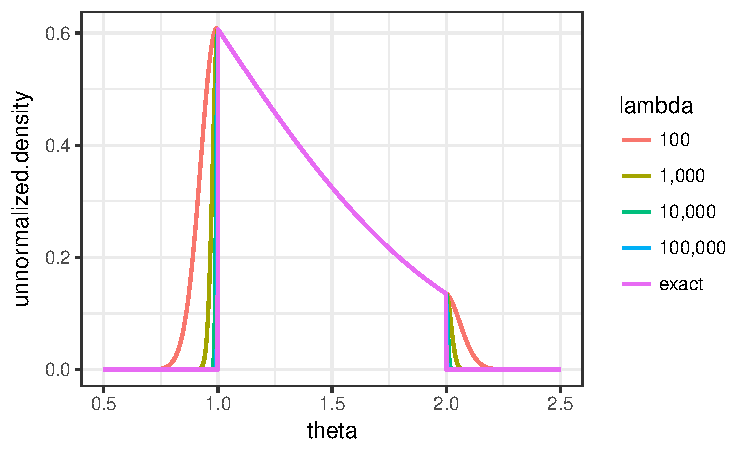
\includegraphics[width=0.5\textwidth]{density_truncated_normal}
\caption{Unnormalized densities for truncated normal $\No_{(1,2)}(0,1)$, under exact and approximating densities. The exact density abruptly drops to $0$ on the two boundaries, while the approximating ones drop continuously. In the approximation, larger $\lambda$ is associated with lower tolerance for constraint violation ($( 1-\theta )_+$ and $( \theta - 2)_+$) in the posterior. All densities inside $(1,2)$ are the same up to a constant difference.}
\label{truncated_normal}
\end{figure}

The kernel specification allows us to obtain strict control of the constraint violation in the posterior. It is attempting to use large $\lambda$ for any model, however, we discover that for model with narrow support on $\mc D$ would have a small step size due to the large $\lambda$. Therefore, in those cases, it is more useful to obtain approximate posterior with moderately small error, then project back to $\mc D$ for exact posterior. More details will be illustrated in the example of next section.

\subsection{Posterior Sampling Under Extrinsic Prior}

We first collect posterior $\pi_K(\theta \mid y)$ under the $\pi_{0,\mc R}(\theta) \pi_K(\theta)$. Since the posterior is defined on a less restrictive $\mc R$, it can be sampled easily. The tradiational sampling approach such as slice sampling, adaptive Metrohepolis-Hastings can be utilized in computation. In this section, we present the sampling algorithm using Hamiltonian Monte Carlo (HMC), due to its high-level automation aided by software and excellent performance in terms of posterior mixing.

In using the conventional HMC, we assume $\mc R$ is an Euchledean space and the constraint functions $E_k(\theta)$'s and $G_k(\theta)$'s  are differentiable with respect to $\theta$. We focus on the case where $\theta$ is continuous, although discrete extension is possible \citep{zhang2012continuous}.

HMC is essentially a data augmentation based Monte Carlo. Using a latent variable ``veolicty'' $p$ that has the same dimension as $\theta$, the total negative log-likelihood-prior function based on \eqref{extrinsic_prior} is

\begin{equation}
\begin{aligned}
H(\theta, p)& = U(\theta)+M(p),\\
\text{where } & U(\theta) = -\log\left\{ L(\theta;y)\pi_{0,\mc R}(\theta) \cdot \prod_{k=1}^{m} K_{1,k}\Big( | E_k(\theta)| \Big) \cdot \prod_{k'=1}^{l} K_{2,k'}\Big( \big( G_{k'}(\theta) \big)_+ \Big) \right\},\\
& M(p) = \frac{p'\Sigma^{-1} p}{2},\end{aligned}
\end{equation}
with $\Sigma^{-1}$ a positive definite matrix and pre-specified as a tuning parameter. Then instead of using conventional updates such as random walk or Gibbs sampling, HMC utilizes the Hamiltonian dynamics that satisfy:

\begin{equation}
\begin{aligned}
\label{hamiltonian}
\frac{\partial \theta (t)}{\partial t} & =\frac{\partial H(\theta, p)}{\partial p} = \Sigma^{-1}p,\\
\frac{\partial p(t)}{\partial t}& =-\frac{\partial H(\theta, p)}{\partial \theta} = -\frac{\partial U(\theta)}{\partial \theta}.
\end{aligned}
\end{equation}

At each step, the current state of $\theta$ is viewed as $\theta(0)$ with $p(0)$ randomly generated from $\No(0, \Sigma)$. Then they enter the Hamiltonian dynamics to generate $\theta(t)$ and $p(t)$. During this process, either exact solution or numerical approximation is obtained. When the solution is exact, the total 
$H(\theta(0),p(0)) = H(\theta(t),p(t))$ and $\theta(t)$ is accepted as the new state for $\theta$ in the Markov chain; when the solution is approximate (commonly via leap-frog method), an additional Metropolis-Hastings step is taken to accept $\theta(t)$ with probability $1\wedge \exp  \left( - H(\theta(t),p(t)) + H(\theta(0),p(0))\right)$. Various adaptive approaches \citep{neal2011mcmc,hoffman2014no} have been developed for making the new state less correlated with the current state. Due to the existence of $\frac{\partial U(\theta)}{\partial \theta}$, the sampling can be carried out easily in common HMC software such as STAN. HMC is geometrically ergodic under very general conditions \citep{livingstone2016geometric}.



Based on \eqref{hamiltonian}, we provide some further intuition on the effect of extrinsic prior in HMC, and guide on selecting the hyper-parameter $\lambda$ from a computing perspective. When $\theta \in \mc D$, extrinsic prior is constant and does not influence the HMC; when $\theta \not \in \mc D$, it provides a space expansion by assigning positive support. The amount of expansion is reversely controlled by $\lambda$. Since the Hamiltonian dynamics \eqref{hamiltonian} is commonly approximated by discrete movement in $\mc R$ (e.g. leap-frog), it is important to ensure the expanded posterior support can be efficently explored in the direction of $\frac{\partial U(\theta )}{\partial \theta}$. For example, when $\mc D$ is a truncated Euchledean space, the gradient $\frac{\partial U(\theta)}{\partial \theta}$ is still efficent for exploring its internal space, so very large $\lambda$ can be used to induce almost no expanded space. However, when $\mc D$ is on a circle, updating along any Euchledean direction will move away from this space. In this case, a smaller $\lambda$ would be better for larger space expansion, allowing HMC to explore more efficently.


\begin{figure}[H]
 \centering
  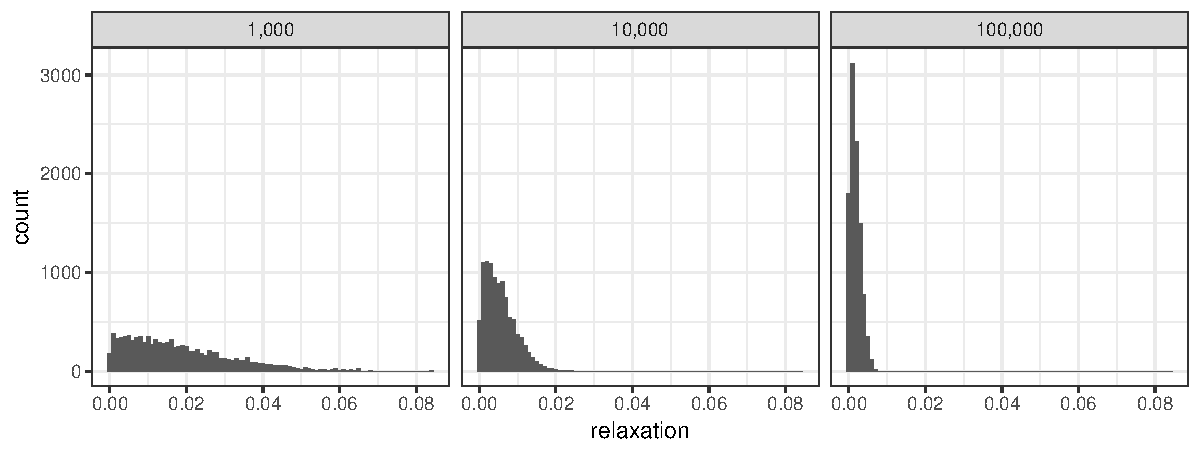
\includegraphics[width=0.8\textwidth]{unit_circle_violation}
 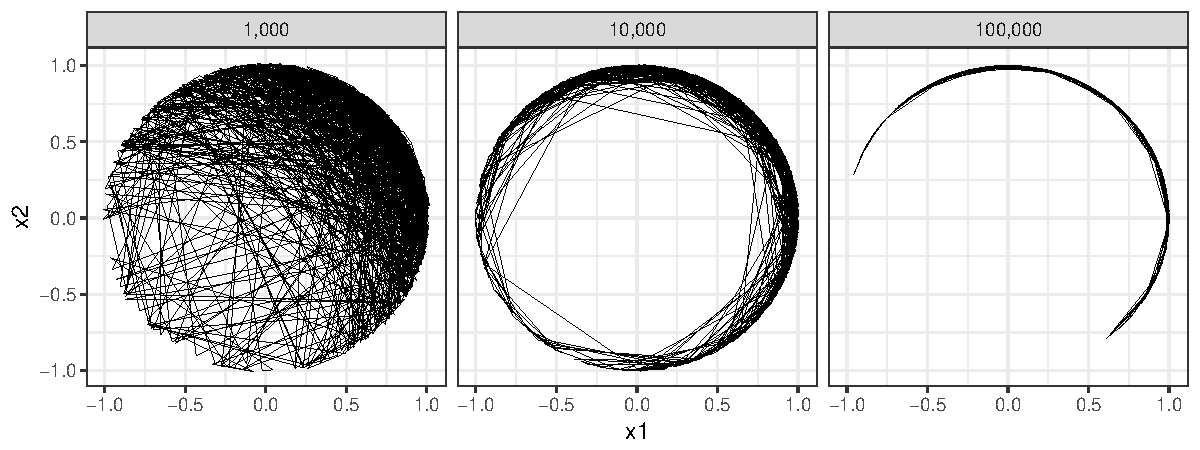
\includegraphics[width=0.8\textwidth]{unit_circle_path}
 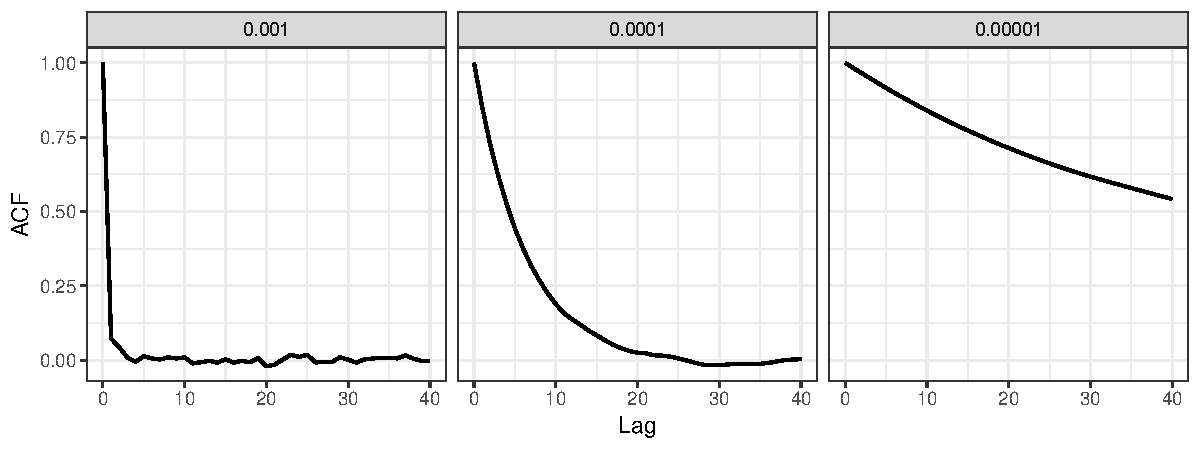
\includegraphics[width=0.8\textwidth]{unit_circle_acf}
\caption{Sampling posterior from a von Mises--Fisher distribution on a unit circle, using HMC with extrinc prior under $\lambda=10^3,10^4,10^5$. Row $1$ shows the posterior distribution of the constraint violation $|\theta'\theta -1|$; Row $2$ shows the sampling path of the Markov chain; Row $3$ shows the autocorrelation plot (ACF). Large $\lambda$ results in small constraint violation, but suffers from slow mixing due to inefficient local update; smaller $\lambda$ increases the approximation error but results in excellent mixing.}
\label{unit_circle}
\end{figure}

To illustrate the latter case, consider generating a random variable $\theta=(x_1,x_2)$ on a unit circle using von Mises--Fisher distribution, $\pi(\theta \mid y) \propto \exp(F'\theta)$ with $\theta'\theta =1$. This is a simple example of a random variable constraint on a $(2,1)$-Stiefel manifold $\mc D =\mc V(2,1)$. We set $F=(1,1)$ to induce a distribution widely spreaded over the manifold, allowing great amount of uncertainty. We use extrinsic prior proportional to $K(\theta)= \exp(-\lambda (\theta'\theta -1)^2) \mathbbm{1}_{|\theta'\theta -1|<0.1}$. Geometrically, the extrinsic prior expands the posterior support from a circle to a ring, with its radius defined by the maximally tolerable constraint violation. 

We tested three different values of $\lambda = 10^3,10^4,10^5$  associated with different radii. For each $\lambda$, we ran HMC for $10,000$ iterations, with $100$ leap-frog steps in each iteration. We use $\Sigma= \diag(1,1)$ to generate velocity. During the initial $2,000$ iterations, we automatically tune the leap-frog step size to obtain an acceptance rate close to $0.6$ in each iteration, then fixed the value for the remaining part of Markov chain. The last $5,000$ iterations are used as posterior samples. Figure~\ref{unit_circle} plots the posterior distribution of constraint violation $|\theta'\theta -1|$, the sampling path and the autocorrelation function (ACF) for each Markov chain. Very large $\lambda=10^5$ has much less constraint violation (hence lower approximation error); however, due to the narrow radius, the associated HMC can only explore local space and results in slow mixing (large autocorrelation even at 40 lags). On the other hand, smaller $\lambda=10^3$ has slightly larger violation (but it is still relatively small), while allows efficient exploration of the space and excellent mixing performance.


\subsection{Correcting Projection to Constraint Space}
 

The posterior sample collected under $\pi_K(\theta \mid y)$ in $\mc R$ is an approximation to $\pi(\theta\mid y)$ in constraint space $\mc D$. One may be interested in further obtaining exact posterior in $\mc D$, likely for two reasons:  (1) to strictly uphold the constraints; (2) to ease the error control in approximate posterior sampling for more efficient computation.

Letting $\theta^*$ be a random sample collected based on $\pi_K(\theta \mid y)$, there exists deterministic projection $M: \mc R\rightarrow \mc D$ and obtain $\theta^*_{\mc D}= M(\theta^*)$. Using this as proposal machineary, one can construct another Markov chain based on $\pi(\theta_{\mc D}  \mid y)$. Letting the current state be $\theta_{\mc D} = M(\theta)$, we generate proposal $\theta^*_{\mc D}= M(\theta^*)$ and accept it with probability:


\begin{equation}
 \begin{aligned}
 1 \wedge \frac{\pi(\theta^*_{\mc D} \mid y) \pi_K(\theta  \mid y) }{\pi(\theta_{\mc D}  \mid y)\pi_K(\theta^* \mid y)}.
 \end{aligned}
 \end{equation}
 This criterion holds since the transformation is deterministic and the posterior collected based on $\pi_K(\theta\mid y)$ is assumed to be independent. Rigoriously speaking, the second condition relies on the geometric convergence of the Markov chain from sampling $\pi_K(\theta \mid y)$, which can be achieved efficiently via algorithm such as HMC.

 The next task is then to optimize the projection. Noting that

\begin{equation}
\begin{aligned}
% |\log( \frac{\pi(\theta^*_{\mc D} \mid y) \pi_K(\theta  \mid y) }{\pi(\theta_{\mc D}  \mid y)\pi_K(\theta^* \mid y)}) | \ge \big| |\log( \pi(\theta^*_{\mc D} \mid y)) - \log( \pi_K(\theta^* \mid y))| - |\log( \pi(\theta_{\mc D} \mid y)) - \log( \pi_K(\theta \mid y))| \big| \\
|\log( \frac{\pi(\theta^*_{\mc D} \mid y) \pi_K(\theta  \mid y) }{\pi(\theta_{\mc D}  \mid y)\pi_K(\theta^* \mid y)}) | \le \big||\log( \pi(\theta^*_{\mc D} \mid y)) - \log( \pi_K(\theta^* \mid y))| + |\log( \pi(\theta_{\mc D} \mid y)) - \log( \pi_K(\theta \mid y))| \big|,
\end{aligned}
\end{equation}
it is sensible to use the projection $\theta_{\mc D}=M(\theta)$ minimizing $Q(\theta_{\mc D})=|\log( \pi(\theta_{\mc D} \mid y)) - \log( \pi_K(\theta \mid y))|$ towards $0$. And the acceptance rate will be close to $1$. This is possible since the extrinsic prior ensures that the approximate $\theta$ is close to $\mc D$ and $\pi(\theta_{\mc D} \mid y) =\pi_K(\theta_{\mc D} \mid y)$. Obviously, when the approximate $\theta \in \mc D$, the optimal projection would be the identity function. When $\theta \not\in \mc D$, standard optimization technique such as KKT multipliers can be used.



\section{Illustration}

{\bf Example 1: Ordered Simplex}

{\bf Example 2: Monotone Spline} 

{\bf Example 3: Orthonormal Gaussian Processes} 

\section{Theory}

posterior propriety

\section{Application}
\section{Discussion}



\bibliography{reference}
\bibliographystyle{chicago}

\end{document}
